\chapter{MARCO TEÓRICO}
\section{MARCO CONCEPTUAL}
\subsection{LeapMotion}
\subsection{Goniometria}
\subsection{Análisis de puesto de trabajo}
\subsection{Enfermedades y lesiones}
\subsubsection{Tenosinovitis De Quervain}
También conocida como tenosinovitis estiloides radiales, consiste en la inflamación de los tendones del pulgar causada por movimientos repetitivos.

Inflamación que produce una estenosis del canal osteofibrososinovial situado en la estiloides radial por el que discurren los tendones del abductor largo y extensor corto del
pulgar. Se produce al combinar agarres con giros o desviaciones cubitales y radiales repetidas o forzadas de la mano
\begin{figure}[H]
    \centering
    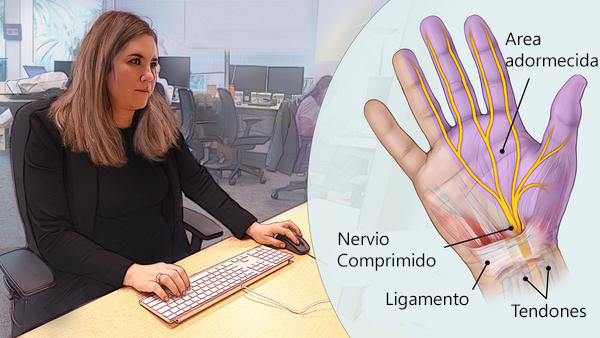
\includegraphics[width=0.7\textwidth]{Anexos/LATEX/chapters/images/STC.jpg}
    \caption{Anatomía de la mano con STC \\\textbf{Fuente:} https://g.co/kgs/BpkB4A}
    \label{STC}
\end{figure}
\subsubsection{Sindrome del Túnel del Carpo}
\paragraph{¿Qué es?}
Existe un espacio en la muñeca llamado túnel del carpo, a través del cual pasan el nervio mediano y nueve tendones flexores que van desde el antebrazo hacia la mano. El Síndrome del Túnel del Carpo (STC) es una condición producida por la compresión del Nervio Mediano, a nivel de la muñeca. Esta compresión produce entumecimiento, hormigueo y dolor en la mano, dedos y ocasionalmente en el brazo. \footcite{SindromeCarpiano}

\begin{figure}[H]
    \centering
    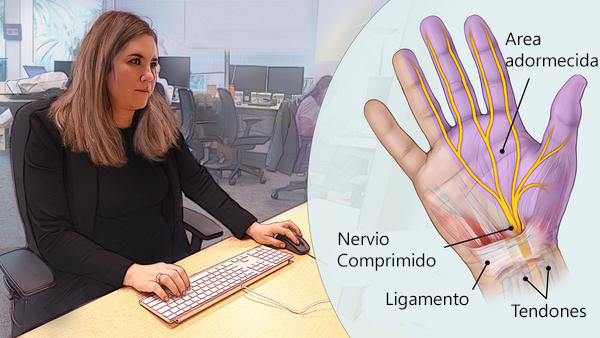
\includegraphics[width=0.7\textwidth]{Anexos/LATEX/chapters/images/STC.jpg}
    \caption{Anatomía de la mano con STC \\\textbf{Fuente:} https://g.co/kgs/MdPBTe}
    \label{STC}
\end{figure}

El STC se presenta cuando se aumenta la presión dentro del túnel por cualquier proceso inflamatorio, comprimiendo el nervio, el cual es una estructura muy sensible a los aumentos de presión. Cuando la presión dentro del túnel es muy alta y altera la función normal del nervio, aparecen rigidez, hormigueo y dolor en la mano y los dedos.\footcite{SindromeCarpiano}
\paragraph{Prevención}
Es recomendable informar al trabajador, entrenándolo para que aquellas posturas o movimientos peligrosos sean evitados durante el desarrollo de su labor, además, el buen diseño de las herramientas, utensilios y del puesto de trabajo ayudan a conseguir la relajación de la mano y de la muñeca.\footcite{SindromeTratarlo}
\subsection{Legislación Vigente}
\section{MARCO REFERENCIAL}
\subsection{Modelos de ergonomía para brazos y muñecas en el contexto nacional}
\subsubsection{Normas GATISO}
\section{Modelos de ergonomía para brazos y muñecas en el contexto internacional}
\subsubsection{}
\section{MARCO TECNOLÓGICO}